\subsubsection{Description}
%Describe the housing used and how it can be accessed, etc.  Describe how the measurement points protected/covered when not in use and how the electrical connections on the back of the measurement points are protected when the measurement points are being used.

\glsreset{tsmp}
\Glspl{tsmp} are placed in the Service box. When not in use, they are covered with protective cups made from silicone rubber. From backside they are protected by heat shrink tube, which prevents moisture from getting in and also accidental touching of high voltage poles.

\subsubsection{Wiring, connectors, cables}
%Describe wiring, show schematics, and describe connectors and cables used and show useful data regarding the wiring.  Include details on the protection resistor including resistance, voltage and power rating.

\Glspl{tsmp} wires will be connected to the Service box, where are terminals connecting Accumulator to Motor controller. There are also 2 resistors 10 k$\Omega$ 5W (R$_1$, R$_2$) wired between those 2 terminals and \glspl{tsmp}. Value of this resistor can be measured from measuring points by multimeter with switched \gls{tsms} off. Service box scheme is shown in \ref{fig:ServiceBox/scheme}.

\begin{figure}[H]
	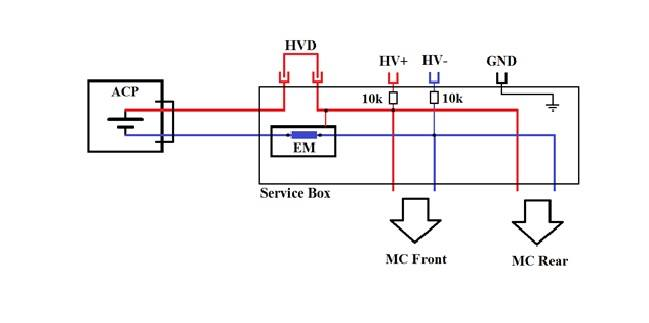
\includegraphics[width=\textwidth]{./img/ServiceBox-scheme.jpg}
	\caption{Service box scheme}
	\label{fig:ServiceBox/scheme}
\end{figure}

\subsubsection{Position in car}
%Provide CAD-renderings showing the relevant parts. Mark the parts in the rendering, if necessary.

Measure points are placed on panel next to Master switches and \gls{hvd}, see \ref{fig:SDC-positionInCar}.